\subsection{\label{sec:A24}Metallischer Lack}
Abschließen führen wir noch THz-TDS-Messungen an mit Nagellack beschichteten Frischhaltefolien 
durch. Hierzu wird zunächst eine unbeschichtete Folie als Referenz-Probe aufgenommen, um die 
Messungen mit den verschiedenen Lackbeschichtungen vergleichbar zu machen. Die Messparameter 
sind für alle Proben identisch und wie folgt gewählt
\begin{equation}
    \Delta s = 0,005\,\si{mm}, \hspace{1.5cm} N_{\text{s}} = 150, \hspace{1.5cm} N_{\text{sample}} = 100, \hspace{1.5cm} s_{0} = 152,7\,\si{mm}.
\end{equation} 
Die reduzierte Schrittweite in Kombination mit der verringerten Schrittzahl, erlaubt es uns schnell den 
Hauptpuls durch die Probe aufzunehmen. \\
Insgesamt vergleichen wir vier Proben mit der Referenzmessung, was vergleichend in Abb.~\ref{fig:lack} 
präsentiert wird. Zunächst werden ein roter und ein magnetischer Nagellack, sowie ein Silberleitlack 
in gleicher Dicke auf die Frischhaltefolie aufgetragen, welche in einen Probenhalter eingespannt wird. 
Um zusätzlich den Einfluss der Dicke zu untersuchen, wird eine weitere Probe unter Verwendung 
des magnetischen Nagellacks hergestellt, die großzügiger aufgetragen wird.
\begin{figure}[h!]
    \centering
    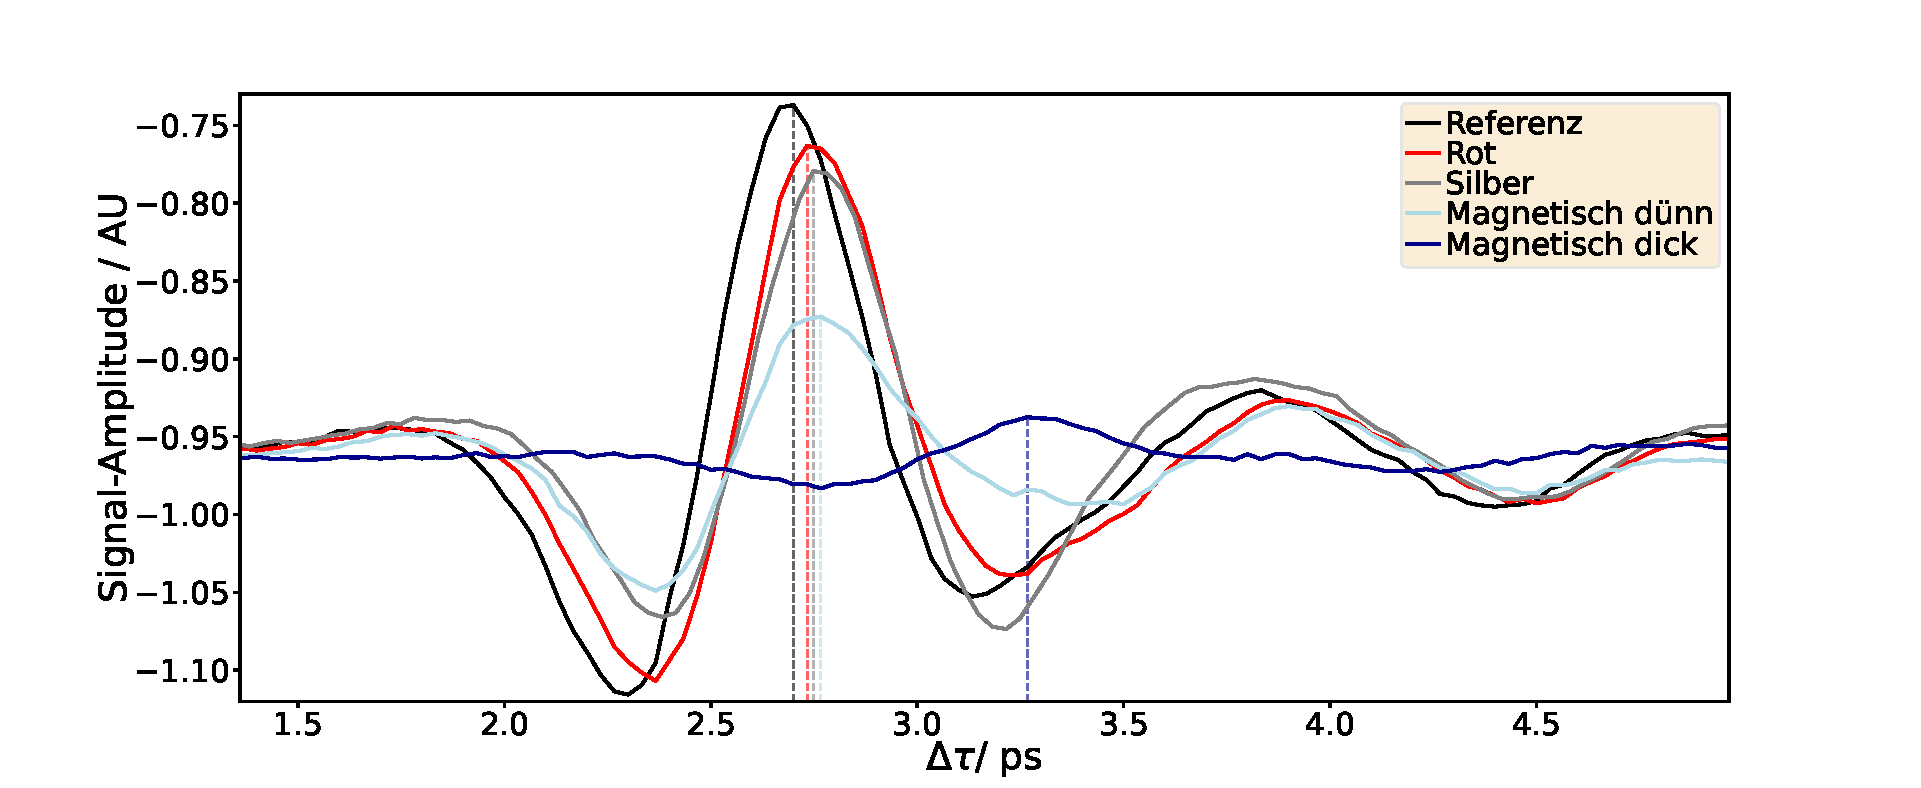
\includegraphics[trim={1.8cm 0.5cm 3.2cm 2.5cm}, clip, width=\textwidth]{Lack.pdf}
    \caption{\label{fig:lack}Das zum E-Feld des THz-Pulses gemessene Spannungssignal als Funktion der 
    zeitlichen Verzögerung $\Delta\tau$ für verschieden beschichtete Proben. Zusätzlich sind vertikale 
    Linien ausgehend von den jeweiligen Amplituden eingezeichnet, um die zeitliche Verzögerung 
    zwischen den Signalen besser abschätzen zu können. Das Darstellungsformat ist bewusst 
    verzerrt gewählt, um die Übersichtlichkeit zu verbessern.}
\end{figure}\FloatBarrier
Zunächst ist zu erkennen, dass jede Probe einen 
zeitlichen Versatz zum Referenzpuls aufweist. 
Dies ist zu erwarten, da der Lack eine zusätzliche 
Schicht darstellt, die einen realen Brechungsindex
unterschiedlich als der von Luft besitzt. Hierdurch ergibt sich
ein zeitlicher Versatz, der in der 
vorbereitenden Frage \ref{subsec:FZV6} beispielhaft
durchgerechnet ist. Da der Versatz proportional zum 
Produkt aus Dicke und Wert des Brechungsindex ist, 
kann man bei gleicher Beschichtungsdicke einen 
Unterschied im Brechungsindex ableiten. 
Für die im Experiment erstellten Proben kann 
jedoch keine einheitliche Schichtdicke garantiert werden.
Erwartungsgemäß ist der Puls, der durch die dicke magnetische Schicht propagiert
am weitesten versetzt. Der Puls, der durch den Silberleitlack 
transmittiert ist, weist sogar einen leicht negativen Versatz auf, was 
auf einen Brechungsindexwert kleiner Eins hinweist. 
Für die benutzte Wellenlänge kann diese Vermutung durch 
Werte aus Datenbanken gestützt werden. Der Hauptbestandteil 
des magnetischen Nagellacks, Eisen, hat in diesem Wellenlängenbereich 
einen deutlich größeren Brechungsindex als Luft, was zu einer Verzögerung des 
Pulses führt. [REF offen]. \\
Zudem sind die Signalamplituden unterschiedlich stark, was 
auf die unterschiedliche Absorption der THz-Strahlung zurückzuführen 
ist. Der rote Lack absorbiert wenig Strahlung, da es sich 
um einen nicht leitenden Stoff handelt. Daher ist eine 
große Bandlücke zu vermuten, zu deren Überwindung die 
Strahlungsenergie nicht ausreicht und eine Wechselwirkung mit freien 
Ladungsträgern aufgrund deren geringer Konzentration nicht zu 
erwarten ist. Der magnetische Nagellack zeigt erwartungsgemäß 
starke Absorption, da die Eisenkügelchen im Lack viele 
freie Ladungsträger besitzt, die mit der Strahlung wechselwirken
können. Die Fermienergie liegt hier im Leitungsband, was 
einen Energieübertrag jeglicher Art ermöglicht und 
damit die Wechselwirkungswahrscheinlichkeit drastisch erhöht. 